\documentclass{article}


\usepackage{PRIMEarxiv}
\usepackage{amsmath}

\usepackage[utf8]{inputenc} % allow utf-8 input
\usepackage[T1]{fontenc}    % use 8-bit T1 fonts
\usepackage{hyperref}       % hyperlinks
\usepackage{url}            % simple URL typesetting
\usepackage{booktabs}       % professional-quality tables
\usepackage{amsfonts}       % blackboard math symbols
\usepackage{nicefrac}       % compact symbols for 1/2, etc.
\usepackage{microtype}      % microtypography
\usepackage{lipsum}
\usepackage{graphicx}
\usepackage{longtable}
\graphicspath{{media/}}     % organize your images and other figures under media/ folder
\renewcommand{\headrulewidth}{0pt}

  
%% Title
\title{Area and Distribution Free Estimators
%%%% Cite as
%%%% Update your official citation here when published 
%\thanks{\textit{\underline{Citation}}: 
%\textbf{Authors. Title. Pages.... DOI:000000/11111.}} 
}

\author{
  Stephen Feldman, \textit{extention of research submitted to:} James Bailey, Bahar \c{C}avdar \\
  Rensselaer Polytechnic Institute \\
  Troy, New York\\
  \texttt{\{feldms5,bailej6,cavdab2\}@rpi.edu} \\
  %% examples of more authors
  % \And
  %Stephen Feldman \\
  %Rensselear Polytechnic Institute \\
  %City\\
  %\texttt{email@rpi.edu} \\
  %% \AND
  %% Coauthor \\
  %% Affiliation \\
  %% Address \\
  %% \texttt{email} \\
  %% \And
  %% Coauthor \\
  %% Affiliation \\
  %% Address \\
  %% \texttt{email} \\
  %% \And
  %% Coauthor \\
  %% Affiliation \\
  %% Address \\
  %% \texttt{email} \\
}

\usepackage{fancyhdr}
\pagestyle{fancy}
\fancyhead{} % This clears all header fields
\fancyhead[LO]{Area and Distribution Free Estimators} % Optional: Put your actual title here
%\fancyhead[LO]{} % Uncomment this line instead if you want the header completely empty
\begin{document}
\maketitle


\begin{abstract}
Efficient estimation of Traveling Salesman Problem (TSP) tour lengths is a prerequisite for scalable logistics planning and Vehicle Routing Problem (VRP) partitioning. However, traditional estimators relying on asymptotic geometric bounds degrade rapidly in high-dimensional or abstract metric spaces relevant to bioinformatics and semantic navigation. This paper introduces an improved Geometrically Assisted Regression Tree (GART 3.0), a dimension-agnostic machine learning estimator that leverages topological invariants derived from the Minimum Spanning Tree (MST) to predict optimal tour lengths in $\mathbb{R}^N$. By discarding computationally expensive geometric features such as the Convex Hull, GART 3.0 achieves maintains high prediction speed in $\mathbb{R}^N$ compared to state-of-the-art solvers (LKH-3) while maintaining a predictive precision of 1.59\% SDPE (Standard Deviation of Percentage Error) on $N$-dimensional benchmarks. Our results demonstrate that Gradient Boosted Regression Trees utilizing topological features match or exceed the accuracy of complex Deep Neural Networks while requiring significantly less computational overhead. Furthermore, we conduct a thorough analysis of existing tour length estimators and adapt them when needed to provide an \textit{N}-dimensional benchmark. Finally, we introduce additional challenging TSP configurations that violate most assumptions of existing estimators. These expose a fundamental robustness gap: unique geometries, especial those that maximize the difference between the bounding box and convex hull, are disruptive to existing estimators.
\end{abstract}


% keywords can be removed
%\keywords{First keyword \and Second keyword \and More}


\section{Introduction}
\label{sec:introduction}

The Traveling Salesman Problem (TSP) asks for the shortest possible route that visits a set of $n$ cities exactly once and returns to the origin. It is a cornerstone of combinatorial optimization. While the problem is NP-hard, the ability to rapidly estimate the optimal tour length $L(S)$ is critical for modern logistics. Estimators allow companies to make quick decisions regarding fleet sizing, clustering, and partitioning for the Vehicle Routing Problem (VRP) without running computationally expensive solvers for every scenario\cite{gart2025}. The economic impact of these estimations is substantial. Last-mile delivery now accounts for approximately 53\% of total shipping costs in supply chains \cite{lastmile2023}. Effective route optimization reduces these operational costs by 15-30\% \cite{paragon2025} and fuel consumption by up to 20\% \cite{finmile2024}. For example, UPS reports that their ORION routing system saves 100 million miles and roughly \$400 million annually \cite{upsorion}. Accurate tour length estimators are the engine behind these savings, enabling systems to evaluate millions of potential route combinations in seconds.

\subsection{Motivation}

Most existing research focuses on the Euclidean plane ($\mathbb{R}^2$) or 3D space. However, this focus excludes a vast class of "pseudo-TSP" problems that operate in high-dimensional or abstract metric spaces. Developing estimators in $\mathbb{R}^N$ serves a practical purpose beyond theory. The Fréchet Embedding Theorem \cite{frechet1906} states that any finite metric space satisfying the triangle inequality can embed into a Banach space ($\ell_\infty$) of sufficient dimension. Similarly, Bourgain \cite{bourgain1985} demonstrates that $n$-point metric spaces map to Euclidean space ($\ell_2$) with low distortion ($O(\log n)$). This allows us to treat abstract problems as geometric TSP instances in $\mathbb{R}^N$. 

Applications of this principle are diverse. In bioinformatics, genetic sequencing often models TSPs on edit-distance graphs \cite{agarwala1996}, which translate into high-dimensional geometric points. In Natural Language Processing (NLP), semantic navigation uses metrics like Word Mover's Distance \cite{kusner2015}. An estimator in $\mathbb{R}^N$ can rapidly predict the "tour length" through semantic concepts. Current 2D estimators rely on properties that fail in high dimensions. For instance, convex hull algorithms become computationally intractable as $N$ increases. This creates a gap in the literature as we lack robust, scalable tools for estimating TSP costs in high-dimensional spaces.

\subsection{Objective and Contributions}

The objective of this project is to develop a library of TSP estimators that maintain accuracy in high-dimensional space. We move beyond geometric formulas and use machine learning to learn the relationship between topological graph features and optimal tour lengths. This paper presents three primary contributions. First, we generate a ground-truth dataset of TSP instances from $d=2$ to $d=5$ using the LKH-3 solver. This provides a baseline for high-dimensional analysis that standard libraries like TSPLIB do not offer.  Second, we extend existing Tour Length Estimation Models to make them compatible with n-dimensional data and benchmark their effectiveness on the data set. We also iteratively test feature and model frameworks to create an efficient Tour Length Estimators that scales well in n-dimensions. Finally, we introduce GART 3.0, a gradient-boosted regressor built dimensional agnostic feature set using LightGBM. It predicts tour lengths in arbitrary dimensions without retraining by learning the ratio between the MST length and the optimal TSP tour.

\subsection{Outline}

The remainder of this report is organized as follows. Section \ref{sec:lit_review} reviews the theoretical limits of classical estimators. Section \ref{sec:methodology} details the data generation pipeline and the architecture of our feature sets. Section \ref{sec:results} benchmarks GART 3.0 against existing tour length estimators, constructive heuristics, and Neural Networks. Finally, Section \ref{sec:conclusion} discusses the implications for solving abstract non-Euclidean TSPs.

\section{Literature Review}
\label{sec:lit_review}

The estimation of Traveling Salesman Problem (TSP) tour lengths is a distinct field of combinatorial optimization that seeks to predict the cost of an optimal solution without incurring the computational expense of exact solvers. Approaches to this problem generally fall into three paradigms: asymptotic geometric analysis, which relies on the statistical properties of point distributions; constructive heuristics, which approximate the tour using tractable graph structures; and simulation-based inference, which estimates the global optimum by sampling local optima. In this section, we survey the specific estimator models implemented in our benchmarking library, defining their mathematical formulations and constants as established in the primary literature.

\subsection{Beardwood-Halton-Hammersley (BHH)}

The theoretical foundation for TSP estimation in Euclidean space is provided by the Beardwood-Halton-Hammersley theorem \cite{bhh1959}. The theorem establishes that for a sequence of independently and identically distributed random variables in $\mathbb{R}^d$, the length of the shortest path converges almost surely as the number of cities $n$ approaches infinity. The estimator posits that the optimal tour length is proportional to the geometric mean of the node density within a bounding region. While theoretically robust for dense, uniform instances ($n \to \infty$), the BHH estimator is notoriously inaccurate for sparse point clouds ($n < 50$) where boundary effects dominate. The standard formulation used in literature for 2-dimensional space is:
\begin{equation}
L_{BHH} = \beta \cdot \sqrt{n \cdot A}
\end{equation}
where $A$ represents the area of the bounding region (typically the minimal bounding box) and $\beta$ is a constant. The value of $\beta$ depends on the distance metric; for Euclidean distances in 2D, the empirically accepted constant is $\beta \approx 0.7124$. Vinel \cite{vinel2018probability} analyzes the BHH estimator in sparse noting that the estimator works well as long normality assumptions hold around 10 nodes at minimum. $L_{Vinel}$ uses the same equation but with the adjusted constant:  $\beta \approx 0.768$ \cite{vinel2018probability}.

\subsection{Chien's Estimator}

To address the limitations of asymptotic theories on finite, sparse graphs, Chien \cite{chien1989} proposed a probabilistic model that explicitly accounts for the discrete nature of connections. Chien's model decomposes the tour cost into two components: a local term representing the connection between neighboring points, and a global term representing the traversal of the geometric area. The estimator was benchmarked specifically on small-to-medium datasets where BHH failed. The precise formulation provided by Chien for planar instances is:
\begin{equation}
L_{Chien} = 2 \cdot D_{avg} + 0.57 \cdot \sqrt{n \cdot A}
\end{equation}
In this equation, $D_{avg}$ denotes the average Euclidean distance from all points to the centroid of the dataset, serving as a proxy for the spatial spread of the nodes. The coefficient $0.57$ is an empirically derived weight that balances the contribution of the area-based density term against the local clustering term.

\subsection{Cavdar and Sokol}

Cavdar and Sokol \cite{cavdarsokol} argued that simple area-based density measures ($A/n$) fail to capture the nuances of spatial distribution, particularly in instances with high aspect ratios or irregular clustering. They introduced a regression-based estimator that replaces the bounding box area with terms derived from the standard deviation of the coordinates. This approach is significantly more robust to outliers. Their model was benchmarked on a wide variety of synthetic distributions, yielding the following regression equation for 2-dimensional instances:
\begin{equation}
L_{Cavdar} = a_0 \cdot \sqrt{n} \cdot \sqrt{\sigma_x \sigma_y} + a_1 \cdot \sqrt{n} \cdot \sqrt{A} \cdot \sqrt{\frac{\sigma_x \sigma_y}{\bar{c}_x \bar{c}_y}}
\end{equation}
Here, $\sigma_x$ and $\sigma_y$ are the standard deviations of the coordinates, and $\bar{c}_x, \bar{c}_y$ are the mean absolute deviations. The coefficients established in their work are $a_0 = 2.791$ and $a_1 = 0.2669$. Furthermore, they observed that the model tends to overestimate costs for very small instances. To counter this, they defined a correction factor $Corr$ to be applied as a divisor ($L_{final} = L_{Cavdar} / Corr$) for $n < 1000$:
\begin{equation}
Corr = 0.9325 \cdot e^{0.00005n} - 0.2972 \cdot e^{-0.0145n}
\end{equation}

\subsection{Vinel's Estimator}

Vinel provides a simplified variation of the BHH equation intended to function as a robust middle ground between the theoretical purity of the asymptotic limit and the complexity of regression models. It eliminates the specific reliance on coordinate variance found in Cavdar's model, returning to a purely volumetric scaling approach but with tuned coefficients for bounded regions. We reformulate the estimator for The estimator is formulated as:
\begin{equation}
L_{Vinel} = b \cdot n^{\frac{d-1}{d}} \cdot V^{\frac{1}{d}}
\end{equation}
For standard uniform distributions in Euclidean space, the scaling constant is set to $b = 0.768$. This estimator relies heavily on the accuracy of the bounding volume $V$ (typically the Convex Hull volume) to serve as a proxy for the feasible region of the tour.

\subsection{MST-Ratio Estimator}

Constructive estimators approximate the optimal tour length $L_{TSP}$ by computing the cost of a related, computationally tractable graph structure. The most fundamental of these is the Minimum Spanning Tree (MST). It is a well-established property of metric spaces that the MST length provides a tight lower bound for the TSP, specifically $L_{MST} \le L_{TSP} \le 2 \cdot L_{MST}$. This stable relationship allows for a simple ratio-based estimator:
\begin{equation}
L_{MST\_Ratio} = \tau \cdot L_{MST}
\end{equation}
The multiplier $\tau$ is empirically derived from Monte Carlo simulations across millions of instances. For 2-dimensional Euclidean problems, the standard value is $\tau = 1.075$. This estimator is particularly valuable because the MST naturally captures the exact topology and clustering of the point cloud, unlike bounding box formulas which can overestimate empty space.

\subsection{Christofides' Algorithm}

While the MST provides a lower bound, Christofides' algorithm \cite{christofides1976} provides a constructive method for generating a guaranteed upper bound. The algorithm works by augmenting the MST with a Minimum Weight Perfect Matching (MWPM) on the set of vertices with odd degrees, denoted as $O$. The union of the MST and the matching forms an Eulerian graph, which can be traversed to form a valid tour. The estimator is defined as:
\begin{equation}
L_{Christo} = L_{MST} + L_{MWPM}(O)
\end{equation}
This approach is computationally more intensive ($O(n^3)$) than the geometric formulas, but it provides a rigorous worst-case guarantee that $L_{Christo} \le 1.5 \cdot L_{OPT}$ for any problem satisfying the triangle inequality.

\subsection{Hilbert Curve Heuristic}

The Hilbert Curve estimator utilizes Space Filling Curves (SFC) to map high-dimensional space into a 1-dimensional representation. First suggested by Bartholdi and Platzman \cite{bartholdi1982n}, this technique is often used in database indexing and provides a fast constructive heuristic for the TSP. The method involves mapping each coordinate $p_i \in \mathbb{R}^d$ to a scalar index $h_i$ on the Hilbert fractal curve. The points are then sorted according to this index. The estimator length is simply the sum of the Euclidean distances between consecutive points in this sorted order:
\begin{equation}
L_{Hilbert} = \sum_{i=1}^{n-1} \|p_{(i)} - p_{(i+1)}\| + \|p_{(n)} - p_{(1)}\|
\end{equation}
where $p_{(i)}$ represents the point at the $i$-th position in the sorted Hilbert sequence. This method effectively preserves the locality of points, ensuring that points close in the N-dimensional space remain close in the 1D ordering. Our implementation uses $p=16$ to provide sufficient resolution to remain computationally tractable.

\subsection{Extreme Value Theory (EVT)}

Simulation-based estimators avoid geometric assumptions entirely by sampling the solution space to infer the global optimum. Golden and Alt \cite{evt_tsp} applied Extreme Value Theory to the TSP, positing that the distribution of local optima found by heuristic search follows a Weibull distribution. The procedure involves generating $k$ independent tours using a fast heuristic (such as 2-Opt) and fitting a Weibull probability density function to the resulting lengths. The estimator is the location parameter $\gamma$, which corresponds to the theoretical minimum of the distribution:
\begin{equation}
L_{EVT} \approx \hat{\gamma} \quad \text{where} \quad f(x; \gamma, \alpha, \beta) = \frac{\alpha}{\beta} \left( \frac{x-\gamma}{\beta} \right)^{\alpha-1} e^{-((x-\gamma)/\beta)^\alpha}
\end{equation}
This method assumes that the sampled local optima are sufficiently representative of the valley containing the global minimum.

\subsection{Basel and Willemain}

Basel and Willemain \cite{baselwillemain} developed a purely statistical estimator that requires no coordinate data, relying solely on the distribution of edge weights in random tours. They hypothesized that the standard deviation of random tour lengths is highly predictive of the gap between the average random tour and the optimal tour. After analyzing a large corpus of instances, they derived the following exponential regression model:
\begin{equation}
L_{Basel} = \exp(1.798 + 0.927 \cdot \ln(\sigma_{rand}))
\end{equation}
Here, $\sigma_{rand}$ is the standard deviation of the lengths of $10,000$ randomly generated tours. This estimator is unique in that it is "blind" to the geometry, operating purely on the statistics of the distance matrix.

\subsection{Machine Learning Approaches}

Recent research has begun to apply machine learning to approximate the optimal tour length. Varol et al. \cite{varol2024} proposed a contextual framework utilizing Deep Neural Networks (DNN) for last-mile delivery applications. Their approach extracts high-dimensional features from the routing graph, specifically transition weight matrices, to train a model that predicts tour costs. The GART framework \cite{gart2025} builds upon this by utilizing Gradient Boosted Regression Trees to predict a multiplicative scaling factor $\alpha$. Rather than predicting the scalar length directly, GART predicts the ratio:
\begin{equation}
\alpha = \frac{L_{TSP}}{L_{MST}}
\end{equation}
This formulation bounds the prediction problem between $1.0$ and $2.0$, creating a scale-invariant target that is significantly easier for machine learning models to learn than the unbounded raw tour length.

\subsection{N-Dimensional Generalization and Adaptations}
\label{subsec:ndim_scaling}

A critical limitation of the classical literature is the implicit assumption of 2-dimensional Euclidean space. Formulas such as Chien's and Cavdar's rely on hard-coded square roots ($\sqrt{Area}$, $\sqrt{n}$), which are dimensionally inconsistent for $d > 2$. To benchmark these estimators in $\mathbb{R}^N$, we derived generalized variants ($L^{Gen}$) based on the principle of dimensional homogeneity.

\subsubsection{Dimensional Scaling Logic}
The tour length $L$ has units of length $[L]^1$. In $d$ dimensions, the bounding hypervolume $V$ has units $[L]^d$. Therefore, the geometric scaling factor must be the $d$-th root of the volume, $V^{1/d}$. Similarly, the Beardwood-Halton-Hammersley theorem establishes that the length of a space-filling curve in $d$ dimensions scales with the node count as $n^{(d-1)/d}$ \cite{bhh1959}.

Based on this derivation, we defined the following generalized estimators for our library:

\begin{itemize}
    \item Generalized Chien\textbf{ ($L_{Chien}^{Gen}$):} We replaced the planar term $\sqrt{n \cdot A}$ with the dimensionally consistent equivalents. The original coefficient ($0.57$) is retained as a baseline weight.
    \begin{equation}
        L_{Chien}^{Gen} = 2 \cdot D_{avg} + 0.57 \cdot n^{\frac{d-1}{d}} \cdot V^{\frac{1}{d}}
    \end{equation}
    
    \item Generalized Cavdar\textbf{ ($L_{Cavdar}^{Gen}$):} The original regression model relies on the product of standard deviations in $x$ and $y$. We generalized this to the geometric mean of standard deviations across all $d$ dimensions. The node scaling $\sqrt{n}$ was replaced by $n^{(d-1)/d}$, and the area term $\sqrt{A}$ by $V^{1/d}$.
    \begin{equation}
        L_{Cavdar}^{Gen} = a_0 \cdot n^{\frac{d-1}{d}} \cdot \left(\prod_{i=1}^{d} \sigma_i\right)^{\frac{1}{d}} + \dots
    \end{equation}
    
    \item Generalized Vinel\textbf{ ($L_{Vinel}^{Gen}$):} The scaling follows the standard asymptotic limit for hypercubes.
    \begin{equation}
        L_{Vinel}^{Gen} = 0.768 \cdot n^{\frac{d-1}{d}} \cdot V^{\frac{1}{d}}
    \end{equation}
\end{itemize}

\subsubsection{Intractability and Exclusions}
While geometric formulas scale efficiently ($O(n)$ or $O(n \log n)$) into high dimensions, constructive and simulation-based estimators face severe computational bottlenecks. For our target benchmark size of $n=10,000$ customers, the following estimators were deemed intractable and excluded from the N-dimensional analysis:

\begin{itemize}
    \item Christofides\textbf{ ($L_{Christo}$):} With a time complexity of $O(n^3)$, computing the Minimum Weight Perfect Matching is infeasible for $n=10,000$ within reasonable experimental time limits.
    \item Simulation Estimators\textbf{ ($L_{EVT}, L_{Basel}$):} These methods require generating thousands of valid tours using 2-Opt heuristics. The cost of running repeated 2-Opt local searches ($O(k \cdot n^2)$) scales poorly, preventing their use in large-scale high-throughput benchmarks.
\end{itemize}

\section{Methodology}
\label{sec:methodology}

To rigorously benchmark the scalability and accuracy of N-dimensional estimators, we constructed a comprehensive synthetic dataset. This dataset was designed to expose estimators to a wide variety of topological structures, ranging from uniform randomness to highly clustered, realistic distributions. We define the generation pipeline, the parametric scope, and the dual-solver protocol used to establish ground-truth tour lengths. All code can be found in the associated \href{https://github.com/sfeldmanMIG25/Area-and-Distribution-Free-Estimators-for-TSP}{GitHub.}

\subsection{Dataset Construction and Ground Truth}

We implemented a custom generation pipeline in Python to create TSP instances with controlled properties. The dataset spans node counts $N \in [5, 1000]$ and dimensions $D \in [2, 5]$. While the theoretical estimators discussed in Section \ref{sec:lit_review} are applicable to arbitrary dimensions ($d \to \infty$), we restricted this study to $d \le 5$. This constraint ensures that we can obtain provably optimal solutions (or high-quality approximations) within reasonable computational timeframes, providing a reliable baseline for error analysis.

\subsubsection{Parametric Distributions}
Real-world TSP instances rarely follow a uniform distribution. To prevent overfitting to "easy" uniform geometries, we generated coordinates using nine distinct distribution families. For an instance with $n$ cities in $d$ dimensions, coordinates were sampled within a grid space $[0, G]^d$ (where $G \in \{100, 1000, 10000\}$) using the following generators:

\begin{itemize}
    \item Uniform \& Normal: The standard baselines. \textit{Uniform} samples points $x \sim U(0, G)$, while \textit{Normal} samples $x \sim \mathcal{N}(G/2, G/6)$, creating a central concentration.
    \item Clustered (Gaussian Mixtures): Simulates "city-cluster" logistics. We generate $\sqrt{n}/4$ centroids and distribute points around them using a variance of $\sigma = 0.05G$.
    \item Cornered \& Ring: Adversarial geometric shapes designed to test convex hull-based estimators. \textit{Cornered} forces points into the extrema of the hypercube, while \textit{Ring} generates a bimodal distribution concentrated on the perimeters.
    \item Grid: A jittered lattice structure where points are placed on a fixed grid with slight Gaussian noise, simulating city blocks.
    \item Power Law: A  distribution where point locations decay exponentially from the center, mimicking scale-free networks.
    \item Correlated N-D: Unlike the previous distributions which generate $d$ independent dimensions, this generator creates dimensions with high covariance, simulating features that are strictly dependent (e.g., elevation correlating with latitude).
\end{itemize}

For every unique combination of $N$, $D$, grid size, and distribution type, we generated 20 distinct random seeds, ensuring statistical significance in the results. Resulting in approximately 40,000 TSP instances.

\subsubsection{Ground Truth Generation}
To evaluate estimator accuracy, we require the "true" optimal tour length $L_{OPT}$. We employed a dual-solver strategy utilizing both exact and heuristic state-of-the-art solvers.

For all instances, we utilized LKH-3 \cite{helsgaun2017}, an implementation of the Lin-Kernighan-Helsgaun heuristic. LKH-3 is widely considered the most effective heuristic for the TSP, capable of finding optimal or near-optimal solutions rapidly. We configured LKH-3 with a dynamic time limit of $t = \max(10, n/10)$ seconds, ensuring sufficient search depth for larger instances ($n > 100$) without stalling the pipeline.

However, heuristics alone cannot guarantee optimality. To validate the LKH-3 results, we employed the Concorde TSP Solver \cite{concorde2006} for all  instances. Concorde uses linear programming relaxations and cutting-plane methods to find the provably exact optimal tour. The optimal solution is chosen based on the shortest tour, and the time is recorded as the lowest time by a solver to achieve the optimal solution.

All distances were computed as explicit integer Euclidean distances (TSPLIB standard) to prevent floating-point rounding errors during solver execution.
\subsection{2D Generalization Benchmark and Adversarial Testing}
\label{subsec:2d_benchmark}

To rigorously test the generalization capabilities of our estimators, particularly their ability to handle unseen topologies, we constructed a separate, dedicated 2D benchmark dataset. Unlike the primary training data, which spans dimensions $d=[2,5]$, this dataset is restricted to the Euclidean plane ($d=2$) but introduces a wider array of exotic and adversarial distributions. This separation ensures that the performance metrics reported for GART 3.0 and other models reflect true generalization rather than memorization of the training distributions.

\subsubsection{Standard Benchmark Configurations}
The base benchmark set consists of instances with node counts $N$ ranging from 5 to 1,000 and grid sizes of $G \in \{1,000, 10,000\}$. To stress-test the estimators against varying degrees of spatial uniformity and centrality, we implemented 11 distinct distribution families beyond the standard Uniform and Normal:

\begin{itemize}
    \item Geometric Transformations: \textit{Triangular} and \textit{Uniform-Triangular} distributions skew the point density towards specific vertices or edges of the grid, testing the estimator's sensitivity to asymmetry.
    \item Centrality Bias\textbf{:} \textit{Squeezed Uniform} and \textit{X-Central} distributions force points into specific geometric sub-regions (e.g., an 'X' shape or a compressed corridor), creating large voids in the bounding box.
    \item Boundary Distributions\textbf{:} The \textit{Boundary} generator places points exclusively near the perimeter of the grid, maximizing the convex hull area relative to the point density.
    \item Scaled Clustering: We implemented a scaling cluster generator that adjusts the cluster radius $r$ dynamically based on the instance size $N$. For large instances ($N=1000$), points are grouped into up to 20 tight clusters with radii as small as $5\%$ of the grid size, simulating highly fragmented logistics networks.
\end{itemize}

A known weakness of classical estimators (e.g., Chien, BHH) is their reliance on the axis-aligned bounding box ($A_{box}$) as a proxy for the feasible region area. For isotropic distributions (like Uniform or Normal), $A_{box}$ correlates well with the Convex Hull area ($A_{hull}$). However, for anisotropic distributions, this correlation breaks down.

To exploit this weakness, we developed the Line Noise distribution. This generator constructs instances where points lie along a single linear vector $\vec{v}$ with slope $m \in [0.2, 5.0]$, subject to perpendicular Gaussian noise $\epsilon \sim \mathcal{N}(0, 0.02G)$.
\begin{equation}
    (x, y) = (t, m \cdot t + b) + \vec{n}_{\perp} \cdot \epsilon
\end{equation}
where $t$ is the position along the line and $\vec{n}_{\perp}$ is the unit normal vector.
This topology creates a "diagonal strip" across the grid. While the axis-aligned bounding box $A_{box} = \Delta x \cdot \Delta y$ remains large (potentially covering the entire grid), the actual area occupied by the points (approximated by $A_{hull}$) is negligible.
\begin{equation}
    A_{box} \gg A_{hull} \approx L_{line} \cdot \sigma_{noise}
\end{equation}
Estimators that rely on $A_{box}$ (including standard BHH implementations) will drastically overestimate the tour length because they assume the points fill the rectangular void. In contrast, topology-aware estimators like GART 3.0 (using MST features) or geometric estimators using explicit Convex Hulls should remain robust, identifying the structure as a linear path rather than a dispersed cloud.

\subsection{Feature Engineering and Complexity Analysis}
\label{subsec:feature_engineering}

To define the inputs for our machine learning estimators, we formalized two distinct feature sets. The selection of these features represents a trade-off between information density and computational tractability, particularly as the dimensionality $d$ increases. We introduce a formal notation $\Phi = \{ \phi_1, \dots, \phi_m \}$ to represent the feature vector extracted from an instance $S$.

\subsubsection{Feature Set V1: Exhaustive Geometric ($\mathcal{F}_{Geo}$)}
Feature Set V1 was designed as a comprehensive baseline for low-dimensional instances ($d \le 3$). It aims to capture every conceivable variation in the point cloud, combining global geometric bounds with intensive iterative clustering metrics.
This set includes:
\begin{itemize}
    \item Hull Geometry\textbf{: }Explicit calculation of the Convex Hull volume and surface area. While highly predictive of the feasible region, the QuickHull algorithm scales as $O(n^{\lfloor d/2 \rfloor})$, making it intractable for $d > 5$.
    \item Spectral Features: Principal Component Analysis (PCA) eigenvalues to detect dimensional collapse (e.g., points on a line).
    \item Clustering Dynamics: We implement a "Two-Pass" clustering feature that compares the partition quality of K-Means against MST-based cuts. This requires iteratively solving the linear sum assignment problem ($O(n^3)$) to align cluster centroids.
\end{itemize}
Due to these complexities, $\mathcal{F}_{Geo}$ is computationally prohibitive for high-throughput estimation in N-dimensional space.

\subsubsection{Feature Set V3: Scalable Topological ($\mathcal{F}_{Topo}$)}
To address the scalability limits of $\mathcal{F}_{Geo}$, we developed Feature Set V3. This set is "dimension-agnostic," relying strictly on graph invariants and statistical moments that require at most $O(n^2)$ time (dominated by the distance matrix calculation). It discards explicit boundary computations (Convex Hulls) in favor of the Minimum Spanning Tree (MST), which remains robust in any metric space. This is the primary feature set used by the GART 3.0 estimator.

\subsubsection{Computational Complexity and Feature Definitions}
Table \ref{tab:feature_complexity} details the complete feature library. We classify features by their computational complexity class in relation to the number of nodes $n$ and dimensions $d$. Note that for $\mathcal{F}_{Topo}$, we strictly exclude any features exceeding $O(n^2)$.

\begin{table}[ht]
\centering
\caption{Feature definitions, notation, and computational complexity. $\mathcal{F}_{Topo}$ (V3) excludes intractable geometric and clustering features.}
\label{tab:feature_complexity}
\resizebox{\textwidth}{!}{%
\begin{tabular}{@{}llcll@{}}
\toprule
\textbf{Category} & \textbf{Feature Notation} ($\phi$) & \textbf{Set} & \textbf{Complexity} & \textbf{Description / Justification} \\ \midrule

\textbf{Global Geometry} 
& $\phi_{Vol}$ (Hypervolume) & All & $O(n \cdot d)$ & Volume of the bounding box defined by $\prod (max_i - min_i)$. \\
& $\phi_{Dens}$ (Node Density) & All & $O(1)$ & Ratio $n / \phi_{Vol}$. Proxies the sparsity of the graph. \\
& $\phi_{Hull}$ (Convex Hull) & $\mathcal{F}_{Geo}$ & $O(n^{\lfloor d/2 \rfloor})$ & Exact volume of the convex hull. \textbf{Intractable in High-D}. \\
& $\phi_{Asp}$ (Aspect Ratio) & All & $O(n \cdot d)$ & Ratio of the largest to smallest coordinate range. \\ \midrule

\textbf{Distribution} 
& $\phi_{Centroid}^{\mu, \sigma}$ & All & $O(n \cdot d)$ & Mean and std. dev. of distances from points to the centroid. \\
& $\phi_{PCA}^{\lambda}$ & $\mathcal{F}_{Geo}$ & $O(d^3)$ & Ratio of first to last PCA eigenvalues. Measures linearity. \\ 
& $\phi_{NN}^{\mu, \sigma}$ & All & $O(n^2)$ & Statistics of the 1st Nearest Neighbor distances. \\ \midrule

\textbf{Graph Topology (MST)}
& $\phi_{MST}^{L}$ (Total Length) & All & $O(n^2)$ & Sum of edge weights in the MST. The primary scaling factor. \\
& $\phi_{MST}^{\mu, \sigma}$ (Edge Stats) & All & $O(n)$ & Mean, std. dev., skew, and kurtosis of MST edge weights. \\
& $\phi_{MST}^{deg}$ (Degree Stats) & All & $O(n)$ & Distribution of vertex degrees in the MST. Proxies "branching". \\
& $\phi_{MST}^{diam}$ (Diameter) & All & $O(n)$ & Weighted diameter of the tree. Measures graph elongation. \\
& $\phi_{Leaf}$ (Leaf Fraction) & All & $O(n)$ & Fraction of nodes with degree 1. Indicates clustering vs. chains. \\ \midrule

\textbf{Clustering}
& $\phi_{K}^{\text{sil}}$ (Silhouette) & $\mathcal{F}_{Geo}$ & $O(n^2)$ & Quality score of K-Means clusters. \\
& $\phi_{K}^{\text{align}}$ (Alignment) & $\mathcal{F}_{Geo}$ & $O(n^3)$ & Alignment error between MST-cuts and Geometric centers. \\ \bottomrule

\end{tabular}%
}
\end{table}

As shown in Table \ref{tab:feature_complexity}, the transition from $\mathcal{F}_{Geo}$ to $\mathcal{F}_{Topo}$ reduces the worst-case complexity from exponential in $d$ ($O(n^{\lfloor d/2 \rfloor})$) to quadratic in $n$ ($O(n^2)$). This reduction is critical for the GART 3.0 framework, allowing it to generate predictions for 10,000-node instances in high-dimensional space in seconds, whereas hull-based estimators would fail to converge.

\subsection{Benchmarking Model Architectures}
\label{subsec:benchmarking_models}

To evaluate the predictive power of Feature Set V1 ($\mathcal{F}_{Geo}$), we implemented a diverse array of regression architectures. These models serve as the baseline for performance, establishing how well the exhaustive feature set can predict the MST-to-TSP ratio $\alpha$ across varying model complexities. All models were trained to predict $\alpha$ rather than the raw tour length $L_{TSP}$, ensuring scale invariance.

\subsubsection{Linear and Polynomial Models}
We implemented three variations of linear regression to test the linearity of the feature space.

\begin{itemize}
    \item Baseline Linear Regression\textbf{ ($M_{Linear}$):} A standard Ordinary Least Squares (OLS) model. To prevent overfitting on high-dimensional features, we applied univariate feature selection using the F-test. Only features with a p-value $< 0.05$ were retained.
    
    \item Boosted Linear Regression\textbf{ ($M_{Boost}$):} This model incorporates "boosted" engineering steps before regression. We applied logarithmic transformations ($\log(1+x)$) to skewed features (e.g., standard deviations, edge weights) and explicitly added interaction terms between clustering metrics (e.g., Silhouette Score $\times$ Cost Ratio). 
    
    \item Piecewise Mixture-of-Experts\textbf{ ($M_{Piece}$):} A "Router-Expert" architecture designed to handle the distinct topological regimes of the TSP. A Decision Tree classifier (depth=1) acts as the router, splitting instances based on the Silhouette Score ($\phi_{K}^{\text{sil}}$). Instances classified as "Clustered" are routed to a specialized linear expert, while "Uniform" instances are routed to a generic "Blob" expert.
    
    \item Polynomial Lasso\textbf{ ($M_{Lasso}$):} To capture non-linear interactions without manual engineering, we employed a pipeline with polynomial feature expansion (degrees 2–3). We utilized LassoCV (L1 regularization) to strictly enforce sparsity, effectively performing automatic feature selection on the generated interaction terms.
\end{itemize}

\subsubsection{Gradient Boosting Machines ($M_{LGBM}$)}
For non-linear modeling, we utilized LightGBM \cite{ke2017lightgbm}, a gradient boosting framework based on decision tree algorithms. Unlike linear models, LightGBM handles categorical features (e.g., Grid Size, Dimension) natively without one-hot encoding, preserving their ordinal information.

Hyperparameter Tuning: We employed the Optuna framework \cite{akiba2019optuna} to perform a Bayesian search over the hyperparameter space. We optimized the number of leaves ($10-30$), maximum depth ($3-8$), and learning rate ($0.01-0.1$) over 50 trials. The objective function minimized the Root Mean Squared Error (RMSE) on a hold-out validation set.

\subsubsection{Neural Network Architectures}
We explored two Deep Neural Network (DNN) architectures implemented in PyTorch to test the efficacy of representation learning.

\begin{itemize}
    \item Standard MLP\textbf{ ($M_{NN}^{v4}$):} A fully connected Multi-Layer Perceptron following the preprocessing strategy proposed by Varol et al. \cite{varol2024}. Continuous features are standardized, and missing values are imputed with zero while adding a binary "indicator" feature for every missing value. The network consists of 2–4 hidden layers with LeakyReLU activations.
    
    \item Two-Tower TabularNet\textbf{ ($M_{NN}^{v6}$):} A state-of-the-art architecture for tabular data inspired by TabTransformer \cite{huang2020tabtransformer}. The model processes continuous and categorical features in separate "towers" (independent MLP blocks) before concatenating their embeddings in a final head. This separation allows the network to learn distinct representations for geometric statistics (continuous) and instance metadata (categorical) before fusion.
\end{itemize}

Both neural architectures were tuned using Optuna to optimize layer width ($64-256$ units), dropout rates ($0.1-0.5$), and learning rates ($10^{-4}-10^{-2}$). Training was performed using the Adam optimizer with early stopping triggered after 20 epochs of no validation improvement.

\subsection{Model Development Using Feature Set V3 ($\mathcal{F}_{Topo}$)}
\label{subsec:v3_benchmarking}

To evaluate the scalability and generalization capabilities of the topological feature set ($\mathcal{F}_{Topo}$), we implemented two distinct modeling architectures. These models were selected to represent the trade-off between high-capacity non-linear approximation and interpretable feature interaction discovery. Unlike the V1 benchmarks, these models are designed specifically to operate without the computational bottleneck of convex hull generation, making them suitable for real-time inference in high-dimensional spaces.

\subsubsection{GART 3.0: LightGBM V3}
The primary candidate for the GART 3.0 estimator is built upon the LightGBM framework, optimized for the V3 feature set. A critical architectural decision in this model is the treatment of the \textit{dimension} feature. While previous iterations treated dimensionality as a categorical variable, GART 3.0 treats it as a continuous numerical regressor. This allows the tree-based model to extrapolate trends to dimensions unseen during training (e.g., training on $d=2..5$ and predicting for $d=50$). The model targets the scale-invariant ratio $\alpha = L_{OPT} / L_{MST}$.

The training protocol utilizes a computationally intensive hyperparameter search via Optuna. We executed 75 trials to optimize the boosting architecture, with a significantly widened search space compared to V1 models. Specifically, we allowed the number of leaves to range from 64 to 512, enabling the model to capture complex topological interactions, while leaving the maximum depth unbounded. Regularization was enforced through L1/L2 penalties ($\lambda \in [10^{-8}, 10.0]$) and aggressive bagging fractions ($0.4-1.0$). To prevent overfitting, we employed early stopping with a patience of 100 rounds. The final model was retrained on the combined training and validation sets using the optimal iteration count derived from the early stopping phase.

\subsubsection{Interpretability Baseline: Lasso Polynomial V3}
To validate the feature interactions within $\mathcal{F}_{Topo}$, we implemented a regularized polynomial regression model using the Lasso (Least Absolute Shrinkage and Selection Operator) algorithm. This model serves as an interpretability baseline, explicitly identifying which topological features drive the tour length estimation. The preprocessing pipeline differs significantly from the tree-based approach. Numeric features are imputed with the median and standardized to zero mean and unit variance, while the \textit{dimension} feature is strictly one-hot encoded to capture dimension-specific intercepts.

Feature engineering is handled automatically via a polynomial expansion of degree 2, generating quadratic terms and pairwise interactions (e.g., $\phi_{MST} \times \phi_{Density}$). This expanded feature space is then fed into a LassoCV regressor with 10-fold cross-validation. The Lasso algorithm applies an L1 penalty to the coefficients, forcing the weights of irrelevant or redundant features to zero. This effectively performs automated feature selection, isolating the specific topological interactions that are statistically significant for predicting tour length.

\subsection{GART 3.0 Model Specification}
\label{subsec:gart3_spec}

The GART 3.0 estimator is defined as a mapping function $f: X_{feat} \to \alpha$, where $X_{feat}$ represents the dimension-agnostic topological feature vector.  Where $X_{feat}$ includes geometric, topological (MST), and distribution features. The model learns the correction factor $\alpha \in [1.0, 2.0]$ required to transform the MST length into the TSP length. Table \ref{tab:gart_features} defines the complete feature space $\mathcal{F}_{Topo}$ used by the model.

\begin{longtable}{p{4cm} p{2.5cm} p{8.5cm}}
\caption{GART 3.0 Feature Definitions ($\mathcal{F}_{Topo}$)} \label{tab:gart_features} \\
\toprule
\textbf{Feature Name} & \textbf{Complexity} & \textbf{Description \& Theoretical Basis} \\
\midrule
\endfirsthead

\toprule
\textbf{Feature Name} & \textbf{Complexity} & \textbf{Description \& Theoretical Basis} \\
\midrule
\endhead

\multicolumn{3}{c}{\textbf{Group 1: Basic Descriptors}} \\
\midrule
\texttt{n\_customers} & $O(1)$ & The number of nodes ($N$) in the instance. Primary scaling factor for path length as defined by the BHH Theorem. \\
\texttt{dimension} & $O(1)$ & The Euclidean dimension ($d$) of the coordinate space. Determines the asymptotic constant $\beta_d$ in the BHH formula. \\
\midrule

\multicolumn{3}{c}{\textbf{Group 2: Geometric Spread (BHH Proxies)}} \\
\midrule
\texttt{bounding\_hypervolume} & $O(N \cdot d)$ & The volume of the hyper-rectangle bounding the points. Used as a computationally cheap proxy for the Convex Hull volume $V$ required by the BHH Theorem. \\
\texttt{node\_density} & $O(1)$ & The density of points within the bounding box ($N / V_{box}$). Proxy for the spatial intensity $\rho(x)$ used in asymptotic analysis. \\
\texttt{aspect\_ratio} & $O(N \cdot d)$ & Ratio of the largest dimension extent to the smallest. Indicates if the instance is "narrow" or "strip-like," which affects the BHH boundary correction terms. \\
\texttt{centroid\_dist\_mean} & $O(N \cdot d)$ & Mean Euclidean distance from points to the geometric centroid. Measures the central tendency of the distribution. \\
\texttt{centroid\_dist\_std} & $O(N \cdot d)$ & Standard deviation of distances to centroid. Indicates dispersion (e.g., uniform vs. clustered around center). \\
\texttt{centroid\_dist\_max} & $O(N \cdot d)$ & Maximum distance to centroid. Approximates the radius of the point cloud. \\
\texttt{centroid\_dist\_iqr} & $O(N \cdot d)$ & Interquartile range of distances to centroid. A robust measure of dispersion unaffected by outliers. \\
\midrule

\multicolumn{3}{c}{\textbf{Group 3: Topological Structure (MST Proxies)}} \\
\midrule
\texttt{mst\_total\_length} & $O(N^2 \cdot d)$ & The sum of all edge weights in the Minimum Spanning Tree. Steele proved this is strictly proportional to $L_{TSP}$ ($L_{TSP} \approx \rho \cdot L_{MST}$), making it the single strongest predictor. \\
\texttt{mst\_edge\_mean} & $O(N)$ & The average weight of an edge in the MST. Represents the characteristic local spacing between neighbors. \\
\texttt{mst\_edge\_std} & $O(N)$ & Standard deviation of MST edge weights. High values indicate variable density (e.g., clusters separated by voids). \\
\texttt{mst\_edge\_skew} & $O(N)$ & Skewness of the edge weight distribution. Positive skew indicates a few very long edges (outliers). \\
\texttt{mst\_edge\_kurtosis} & $O(N)$ & Kurtosis of edge weights. Measures the "tailedness" of the local distance distribution. \\
\texttt{mst\_edge\_max} & $O(N)$ & The longest single edge in the MST. Often corresponds to the "bottleneck" distance between distinct clusters. \\
\texttt{mst\_edge\_q10--q90} & $O(N \log N)$ & Percentiles (10, 25, 50, 75, 90) of MST edge weights. Captures the transition from dense sub-clusters to sparse global connectivity. \\
\texttt{mst\_degree\_mean} & $O(N)$ & Average vertex degree in the MST. For any tree, this is always $2(N-1)/N \approx 2$. Included for consistency. \\
\texttt{mst\_degree\_std} & $O(N)$ & Standard deviation of vertex degrees. High deviation indicates "hub" nodes (star-like topology) versus "path-like" topology. \\
\texttt{mst\_degree\_max} & $O(N)$ & Maximum vertex degree in the MST. Identifies central hubs. A high max degree correlates with a higher TSP/MST ratio. \\
\texttt{mst\_diameter} & $O(N)$ & The length (number of edges) of the longest path in the MST. Distinguishes "stringy" graphs (high diameter) from "compact" graphs (low diameter). \\
\texttt{large\_edge\_count} & $O(N)$ & Count of edges exceeding $\mu + \sigma$. A proxy for the number of distinct clusters or separations in the instance. \\
\bottomrule
\end{longtable}

\subsubsection{Hyperparameter Tuning and Configuration}

The LightGBM model configuration was selected to balance high model complexity with aggressive regularization. This approach allows the model to capture non-linear interactions between topological features while preventing overfitting on the geometric noise inherent in random graphs. 

\paragraph{Hyperparameter Configuration}
Table \ref{tab:hyperparams} details the optimal hyperparameters identified during the tuning process.

\begin{longtable}{p{3.5cm} p{2cm} p{9cm}}
\caption{Optimal Hyperparameter Configuration (V3)} \label{tab:hyperparams} \\
\toprule
\textbf{Hyperparameter} & \textbf{Value} & \textbf{Description \& Role} \\
\midrule
\endfirsthead

\toprule
\textbf{Hyperparameter} & \textbf{Value} & \textbf{Description \& Role} \\
\midrule
\endhead

\texttt{learning\_rate} & 0.0128 & \textbf{Step Size.} A low learning rate (approx. 1.2\%) forces the model to learn slowly using thousands of trees, ensuring robust convergence and generalization. \\
\texttt{num\_leaves} & 142 & \textbf{Tree Complexity.} Defines the maximum number of leaves per tree. While lower than the upper bound of the search space, 142 is significantly higher than the default (31), allowing the capture of complex interactions between MST structure and point density. \\
\texttt{lambda\_l1} & $8.49 \times 10^{-8}$ & \textbf{L1 Regularization.} The optimizer converged to a negligible L1 penalty, indicating that sparsity (feature selection via lasso-style regularization) was less critical than weight smoothing for this dataset. \\
\texttt{lambda\_l2} & 1.4318 & \textbf{L2 Regularization.} A moderate L2 penalty restricts the magnitude of leaf weights, preventing any single node from dominating predictions and reducing sensitivity to outliers. \\
\texttt{feature\_fraction} & 0.6575 & \textbf{Column Subsampling.} Each tree is constructed using $\approx 66\%$ of the available features. This reduces correlation between trees and prevents over-reliance on dominant features like \texttt{centroid\_dist\_std}. \\
\texttt{bagging\_fraction} & 0.4324 & \textbf{Row Subsampling.} Each tree sees only $\approx 43\%$ of the training instances. This aggressive bagging strategy significantly increases ensemble diversity and reduces variance. \\
\texttt{bagging\_freq} & 5 & \textbf{Bagging Frequency.} Performing row subsampling (bagging) every 5 iterations. \\
\texttt{min\_child\_samples} & 22 & \textbf{Leaf Stability.} A lower threshold for data samples per leaf allows the model to capture finer local patterns in the feature space without fitting pure noise. \\
\texttt{n\_estimators} & 3,224 & \textbf{Number of Trees.} Determined dynamically via early stopping to minimize validation RMSE. \\
\bottomrule
\end{longtable}

The hyperparameters were optimized using Optuna, a Bayesian optimization framework, employing a two-stage strategy to maximize efficiency and performance.

\begin{enumerate}
    \item Stage 1: Bayesian Optimization Search. The initial search focused on exploring the hyperparameter space to minimize the Root Mean Squared Error (RMSE) on a stratified validation set. The process involved 75 trials, exploring a wide range of values for complexity (e.g., \texttt{num\_leaves} $\in [64, 512]$) and regularization. Unpromising trials were pruned efficiently using early stopping with a patience of 100 rounds.
    \item Stage 2: Final Model Refinement. Once the optimal hyperparameters were identified, a final refinement step was executed. First, a temporary model was trained using the best parameters and a high ceiling for \texttt{n\_estimators} (5000). Early stopping pinpointed the validation loss stabilization point. Second, the final production model was retrained on the combined dataset (Training + Validation) using the discovered hyperparameters and the optimal number of trees.
\end{enumerate}

Post-training analysis of the final estimator (V3) highlights the computational depth required to approximate the $\alpha$ constant accurately. The ensemble converged at 3,224 trees, containing a total of 457,808 leaves and 454,584 decision splits across the entire forest. The average prediction complexity is approximately 33,148\textbf{ }operations (splits) per inference. This indicates a high-fidelity model that leverages deep interaction checks to distinguish between subtle variations in graph topology.


\section{Results}
\label{sec:results}
In this section, we evaluate the performance of the proposed estimators across three critical dimensions: computational speed, predictive precision, and robustness to high-dimensional topology. The analysis begins by quantifying the computational efficiency of each model, establishing which estimators are viable for real-time applications. We then assess predictive accuracy using the coefficient of determination ($R^2$) and the Standard Deviation of Percentage Error (SDPE), prioritizing consistency over raw bias. Finally, we examine the generalization capabilities of the models on the  "Line Noise" dataset and their scalability into $N$-dimensional space.

\subsection{Computational Efficiency and Timing Analysis}
\label{subsec:timing_analysis}

The primary constraint for a practical Tour Length Estimator (TLE) is that it must be significantly faster than running an exact solver or a high-quality heuristic. To quantify this, we decomposed the total prediction time $T_{pred}$ for machine learning models into two components:
\begin{equation}
    T_{pred} = T_{feat} + T_{inf}
\end{equation}
where $T_{feat}$ is the time required to compute the feature vector from raw coordinates, and $T_{inf}$ is the inference latency of the model (e.g., tree traversal for LightGBM).

Table \ref{tab:timing_results} summarizes the average computational costs for the benchmarked estimators across the 2D dataset. The average optimal solve time (using Concorde/LKH-3) for this dataset was 9.53 seconds.

\begin{table}[ht]
\centering
\caption{Average Computational Time (Seconds) by Model Type. $T_{feat}$ and $T_{inf}$ are reported for ML models where applicable.}
\label{tab:timing_results}
\resizebox{\textwidth}{!}{%
\begin{tabular}{@{}lccccr@{}}
\toprule
\textbf{Model / Method} & \textbf{Type} & \textbf{Feature Time ($T_{feat}$)} & \textbf{Inference Time ($T_{inf}$)} & \textbf{Total Time ($T_{pred}$)} & \textbf{Speedup vs. Solver} \\ \midrule
\multicolumn{6}{c}{\textit{Optimal Solver Baseline}} \\ \midrule
\textbf{LKH-3 / Concorde} & Exact/Heuristic & - & - & \textbf{9.5267 s} & 1.0x \\ \midrule
\multicolumn{6}{c}{\textit{Geometric \& Constructive Estimators}} \\ \midrule
Chien & Formula & - & - & 0.0036 s & 2,625x \\
Vinel & Formula & - & - & 0.0064 s & 1,488x \\
BHH Asymptotic & Formula & - & - & 0.0082 s & 1,159x \\
Hilbert Curve & Constructive & - & - & 0.0336 s & 283x \\
MST Ratio & Constructive & - & - & 0.0754 s & 126x \\ \midrule
\multicolumn{6}{c}{\textit{Machine Learning Estimators (GART Series)}} \\ \midrule
\textbf{GART 1.0 (V1)} & LightGBM & 0.1330 s & 0.0305 s & \textbf{0.1635 s} & \textbf{58x} \\
\textbf{GART 2.0 (V1)} & LightGBM & 1.1414 s & 0.0209 s & 1.1624 s & 8.2x \\
\textbf{GART 3.0 (V3)} & LightGBM & 0.2892 s & 0.0451 s & \textbf{0.3343 s} & \textbf{28x} \\
Lasso Poly V3 & Linear & 0.3813 s & 0.0451 s & 0.4264 s & 22x \\ \midrule
\multicolumn{6}{c}{\textit{Deep Learning Benchmarks}} \\ \midrule
NN v4 (Varol) & MLP & 1.1869 s & 0.0506 s & 1.2374 s & 7.7x \\
NN v6 (Two-Tower) & Transformer & 1.3494 s & 0.0814 s & 1.4308 s & 6.6x \\ \bottomrule
\end{tabular}%
}
\end{table}

\subsubsection{Timing Analysis and Feature Overhead}
The results highlight a critical trade-off between feature complexity and prediction speed.

1.  Geometric Formulas are near instantaneous: Classical formulas like Chien and Vinel operate in milliseconds ($<0.01s$), effectively zero-cost. However, as shown in later sections, their precision is often insufficient for routing optimization.

2.  Feature Extraction Bottleneck: For the ML models, feature calculation ($T_{feat}$) dominates the total time, accounting for $80-98\%$ of latency.
    \begin{itemize}
        \item GART 1.0 is the fastest ML model ($0.16s$), benefiting from using only 15 features and the optimized library for ConvexHull\cite{gart2025}.
        \item GART 3.0 (V3 Features) shows a slight increase in computational cost ($0.33s$) compared to GART 1.0. This is attributable to the replacement of the Convex Hull ($O(N \log N)$) with more intensive spectral graph features derived from the MST, which are necessary to maintain robustness in $N$-dimensions where Convex Hulls fail. Despite this, GART 3.0 maintains a 28x speedup over the solver.
        \item Neural Networks: The Neural Network models (v4/v6) incurred significantly higher overhead ($>1.2s$), largely due to additional manipulations to each feature set.
    \end{itemize}

\subsubsection{Scalability with Problem Size ($N$)}
The stability of the estimator runtimes as the number of customers $N$ increases is illustrated in Figure \ref{fig:time_vs_n_200}.

\begin{figure}[ht]
    \centering
    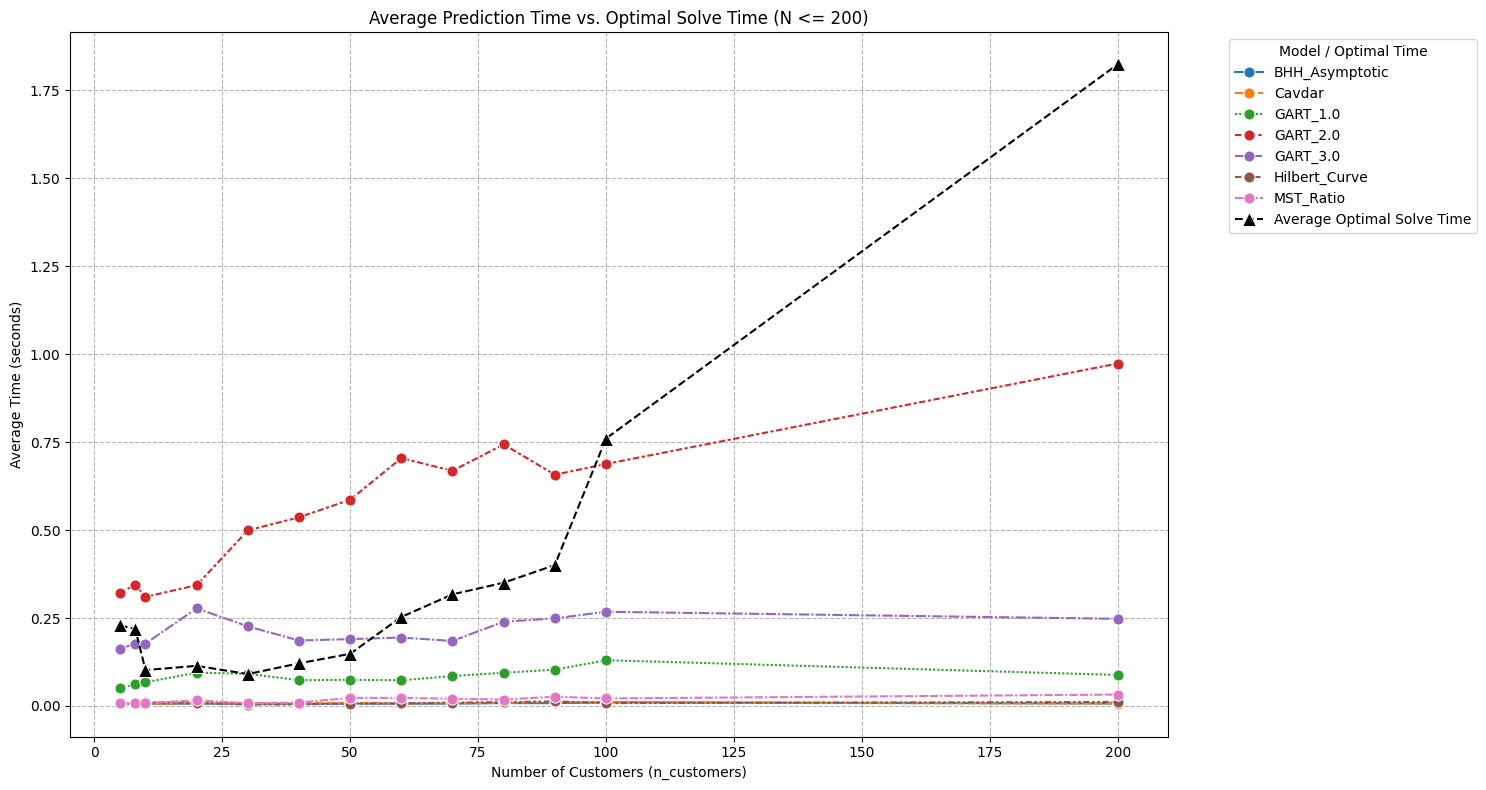
\includegraphics[width=1\linewidth]{avg_predict_2d_n200.png}
    \caption{Scalability Analysis ($N \le 200$): Comparison of estimator prediction times against the optimal solver}
    \label{fig:time_vs_n_200}
\end{figure}

As $N$ approaches 200, the optimal solver time begins to spike, reflecting the NP-hard nature of the TSP. In contrast, the GART estimators scale polynomially (primarily $O(N^2)$ due to the distance matrix computation), appearing nearly constant on this scale.

Figure \ref{fig:time_vs_n_filtered} expands this view to $N=1000$.

\begin{figure}[ht]
    \centering
    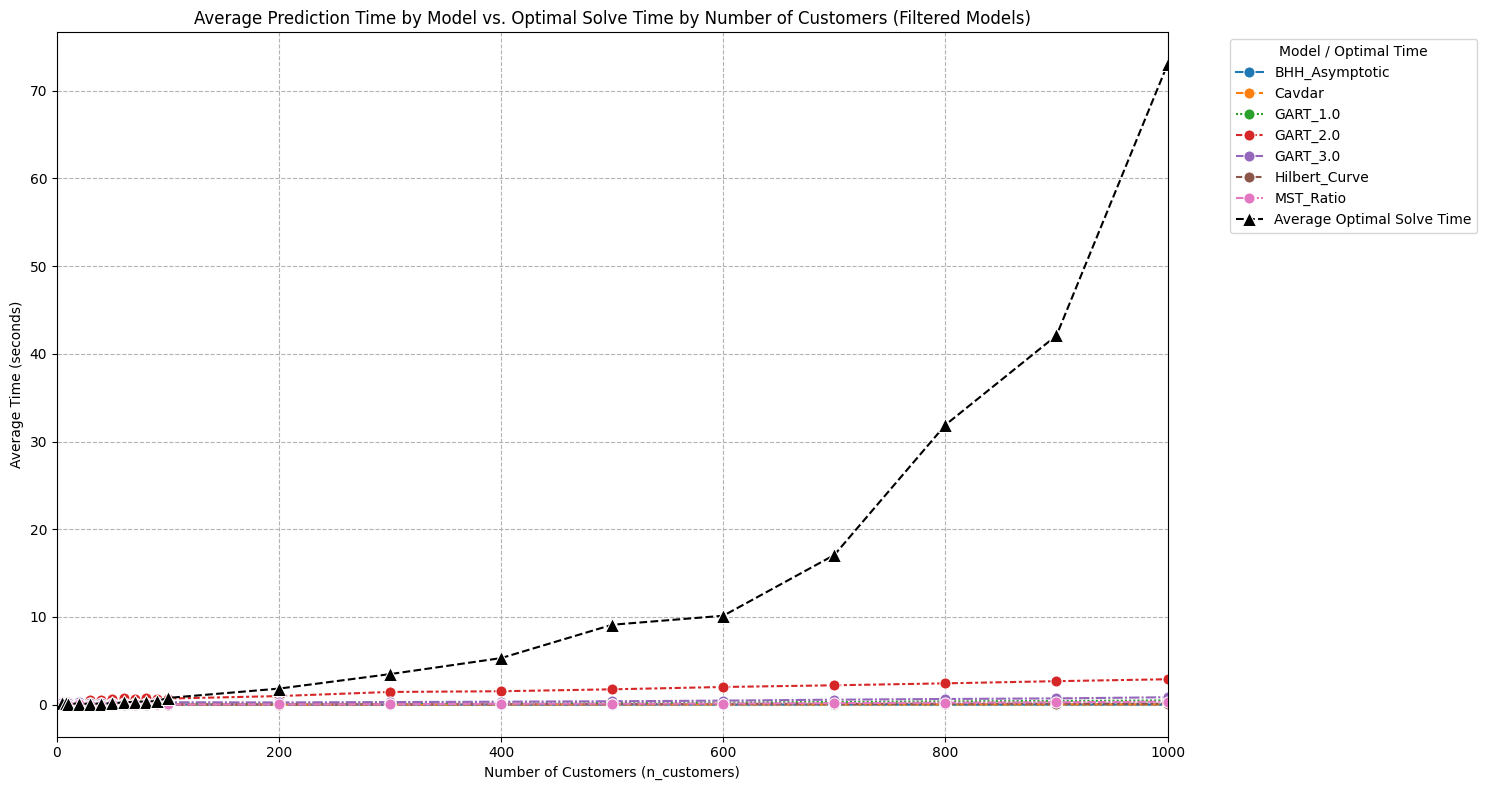
\includegraphics[width=1\linewidth]{avg_predict_2d.png}
    \caption{Long-Range Scalability ($N \le 1000$)}
    \label{fig:time_vs_n_filtered}
\end{figure}

The exhaustive feature sets (used in GART 2.0 and the Neural Networks) show a noticeable cost penalty in Figure \ref{fig:time_vs_n_filtered} (red line), approaching 2-3 seconds at $N=1000$. GART 3.0 (purple), by stripping away intractable geometric features, maintains a highly favorable profile, staying well below the 1-second threshold required for real-time interactive planning systems.

\subsubsection{Scalability with Dimensionality}
\label{subsec:ndim_scalability}

To verify that our estimators remain efficient as problem complexity increases, we analyzed the prediction latency across the N-dimensional dataset ($d \in \{2, 3, 4, 5\}$). Figure \ref{fig:nd_facet} presents a facet grid of prediction times, isolating the impact of dimensionality.

\begin{figure}[ht]
    \centering
    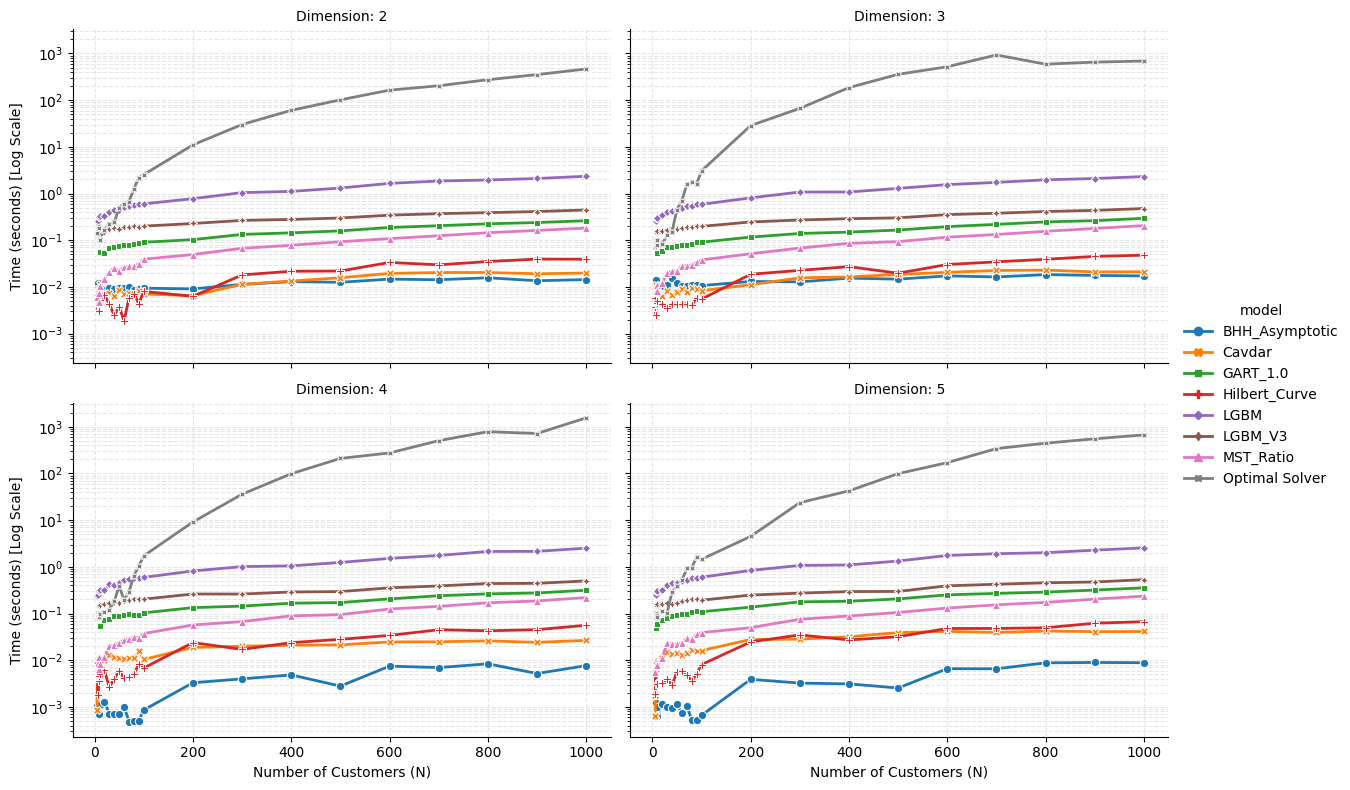
\includegraphics[width=1\linewidth]{ND_facet_grid.png}
    \caption{N-Dimensional Prediction Latency ($d \in [2,5]$):}
    \label{fig:nd_facet}
\end{figure}

Table \ref{tab:ndim_timing} details the computational profile of the estimators on the N-dimensional dataset. With the increased complexity of higher-dimensional solving, the average ground-truth generation time rose to 212.59 seconds, amplifying the relative speedup of the estimators.

\begin{table}[ht]
\centering
\caption{N-Dimensional Computational Efficiency ($d \in [2,5]$). Speedup is calculated relative to the average optimal solver time of 212.59s.}
\label{tab:ndim_timing}
\resizebox{\textwidth}{!}{%
\begin{tabular}{@{}lccccr@{}}
\toprule
\textbf{Model / Method} & \textbf{Type} & \textbf{Feature Time ($T_{feat}$)} & \textbf{Inference Time ($T_{inf}$)} & \textbf{Total Time ($T_{pred}$)} & \textbf{Speedup vs. Solver} \\ \midrule
\multicolumn{6}{c}{\textit{Optimal Solver Baseline}} \\ \midrule
\textbf{LKH-3 / Concorde} & Exact/Heuristic & - & - & \textbf{212.5921 s} & 1.0x \\ \midrule
\multicolumn{6}{c}{\textit{Geometric \& Constructive Estimators}} \\ \midrule
Chien & Formula & - & - & 0.0073 s & 29,122x \\
BHH Asymptotic & Formula & - & - & 0.0096 s & 22,145x \\
Vinel & Formula & - & - & 0.0135 s & 15,748x \\
Hilbert Curve & Constructive & - & - & 0.0226 s & 9,407x \\
MST Ratio & Constructive & - & - & 0.0871 s & 2,441x \\ \midrule
\multicolumn{6}{c}{\textit{Machine Learning Estimators (GART Series)}} \\ \midrule
\textbf{GART 1.0 (V1)} & LightGBM & 0.1316 s & 0.0268 s & \textbf{0.1584 s} & \textbf{1,342x} \\
\textbf{GART 3.0 (V3)} & LightGBM & 0.2702 s & 0.0200 s & 0.2902 s & \textbf{732x} \\
Lasso Poly V3 & Linear & 0.2250 s & 0.0153 s & 0.2403 s & 885x \\ \midrule
\multicolumn{6}{c}{\textit{Deep Learning Benchmarks}} \\ \midrule
NN v4 (Varol) & MLP & 1.1186 s & 0.0548 s & 1.1734 s & 181x \\
NN v6 (Two-Tower) & Transformer & 1.1376 s & 0.0923 s & 1.2299 s & 172x \\ \bottomrule
\end{tabular}%
}
\end{table}

\paragraph{Analysis of Dimension Scalability}
The results reveal a notable finding regarding the trade-off between geometric and topological feature engineering. Counter-intuitively, GART 1.0 \cite{gart2025} remains faster than GART 3.0 (V3 Features) in this specific regime ($d \le 5$).

\begin{itemize}
    \item GART 1.0 Avg Time: 0.158s (Speedup: 1,342x)
    \item GART 3.0 Avg Time: 0.290s (Speedup: 732x)
\end{itemize}

This discrepancy is explained by the 25 features of the V3 feature set. GART 1.0 relies on the Convex Hull, which is calculated via the QuickHull algorithm. In low dimensions ($d \le 5$), QuickHull is highly efficient ($O(n \log n)$). However, GART 3.0 was explicitly designed to function without the Convex Hull to survive in high dimensions ($d \gg 10$). To compensate for the loss of the hull boundary, GART 3.0 computes richer spectral and MST-based features (e.g., tree diameter, eigenvalues), which incur a higher constant computational cost ($T_{feat} \approx 0.27s$) compared to the 15 features in GART 1.0.

While GART 3.0 is slightly slower than its predecessor in low dimensions, it still offers a massive 732x speedup over the solver. More importantly, unlike GART 1.0, it is theoretically capable of scaling to $d=100$ where hull-based methods would become intractable. Future work will extend this benchmark to hyper-dimensional spaces to pinpoint the "crossover" dimension where GART 3.0 becomes the faster alternative.

\subsection{Predictive Precision and Model Quality Assessment}
\label{subsec:precision_analysis}

Having established the computational cost of each estimator, we now evaluate their predictive quality. To prioritize consistency over raw bias (which can be corrected via simple calibration), we utilize the Standard Deviation of Percentage Error (SDPE) as our primary metric of precision, alongside the Coefficient of Determination ($R^2$) to measure structural correlation.

Table \ref{tab:precision_results} presents the performance metrics across both the 2D and N-Dimensional benchmarks. Note that \textit{Mean Bias} is excluded from this discussion, as a non-zero bias with low SDPE represents a consistent, correctable offset, whereas high SDPE indicates irreducible variance.

\begin{table}[ht]
\centering
\caption{Model Precision Metrics ($R^2$ and SDPE)}
\label{tab:precision_results}
\resizebox{\textwidth}{!}{%
\begin{tabular}{@{}llcc|cc@{}}
\toprule
& & \multicolumn{2}{c|}{\textbf{2D Benchmark (Including Linear Noise Cases}} & \multicolumn{2}{c}{\textbf{N-Dimensional Benchmark}} \\
\textbf{Model} & \textbf{Type} & \textbf{$R^2$ Score} & \textbf{SDPE (\%)} & \textbf{$R^2$ Score} & \textbf{SDPE (\%)} \\ \midrule
\textbf{GART 3.0} & \textbf{Tree Ensemble} & \textbf{0.9969} & \textbf{6.14} & \textbf{0.9999} & \textbf{1.59} \\
NN v6 (Two-Tower) & Deep Learning & 0.9972 & 5.31 & 0.9999 & 1.66 \\
NN v4 (Varol) & Deep Learning & 0.9980 & 5.37 & 0.9999 & 1.77 \\
Lasso Poly V3 & Linear & 0.9967 & 7.50 & 0.9997 & 4.00 \\
GART 1.0 & Tree Ensemble & 0.9881 & 7.95 & 0.9722 & 7.96 \\ \midrule
\multicolumn{6}{c}{\textit{Constructive \& Geometric Baselines}} \\ \midrule
MST Ratio & Constructive & 0.9923 & 11.06 & 0.9964 & 8.43 \\
Cavdar & Regression & 0.9089 & 42.04 & 0.9309 & 44.08 \\
Chien & Geometric & 0.8738 & 42.55 & 0.6714 & 84.41 \\
BHH Asymptotic & Geometric & 0.9429 & 32.05 & 0.6734 & 95.96 \\ \bottomrule
\end{tabular}%
}
\end{table}

\subsubsection{The Failure of Classical Estimators}
The results definitively show that classical geometric estimators (Chien, BHH, Cavdar) are insufficient for high-fidelity routing applications. In 2D, even the distribution free regression model by Cavdar yields an SDPE of $42.04\%$. In N-dimensions, this degradation accelerates, with BHH and Chien dropping to $R^2 < 0.70$ and SDPE approaching $100\%$. This confirms that asymptotic density assumptions fail to capture the structural nuances of finite ($N \le 1000$) point clouds.

\subsubsection{GART 3.0 vs. Deep Learning: The Efficiency Frontier}
The machine learning models exhibit a quantum leap in precision, with $R^2$ scores consistently exceeding $0.99$. 
In the 2D Benchmark, the "Heavy" Neural Networks (NN v4/v6) achieve the lowest dispersion ($SDPE \approx 5.3\%$), slightly edging out GART 3.0 ($6.14\%$). However, referring back to the timing analysis, these NNs require over $1.2$ seconds per prediction. GART 3.0 achieves nearly identical precision ($R^2$ difference of $0.0003$) while running 4x faster than the NNs.

In the N-Dimensional Benchmark, GART 3.0  outperforms the Neural Networks, achieving an SDPE of 1.59\% compared to 1.66\% for the Two-Tower architecture. This suggests that the tree-based architecture of GART 3.0 is more effective at partitioning the high-dimensional feature space than the continuous manifolds learned by the MLPs, likely due to the sharp decision boundaries inherent in decision trees.

\subsubsection{Validation of the Topological Feature Set (V3)}
A key finding is the performance divergence between GART 1.0 and GART 3.0 (V3) in N-dimensions. GART 1.0, which relies on the Convex Hull, sees its $R^2$ drop to $0.972$ in high-dimensional space. GART 3.0, utilizing the scalable MST-centric feature set, improves to $0.9999$. This confirms that topological invariants (like MST diameter and spectral gaps) are far more robust predictors of tour length in $\mathbb{R}^N$ than geometric bounds, which suffer from the "curse of dimensionality" where volumes become sparse and meaningless.

While GART 3.0 demonstrates exceptional precision on the standard test set, these results are derived from the same distribution families (Uniform, Cluster, etc.) used during training. The transition from V1 to V3 involved removing the Convex Hull. Theoretically, this removal leaves the model vulnerable to linear topologies where the MST length is small but the spatial extent is large. To probe this potential weakness, we proceed analyze the impact of the unseen "Line Noise" distribution dataset.

\subsection{Generalization to Adversarial Topologies}
\label{subsec:adversarial_analysis}

To rigorously test the robustness of the estimators against non-uniform manifolds, we evaluated their performance on the "Line Noise" dataset. This topology, illustrated in Figure \ref{fig:line_noise_example}, represents a worst-case scenario for geometric estimators: the point cloud is confined to a 1D diagonal strip, yet the axis-aligned bounding box covers the entire 2D grid area.

\begin{figure}[ht]
    \centering
    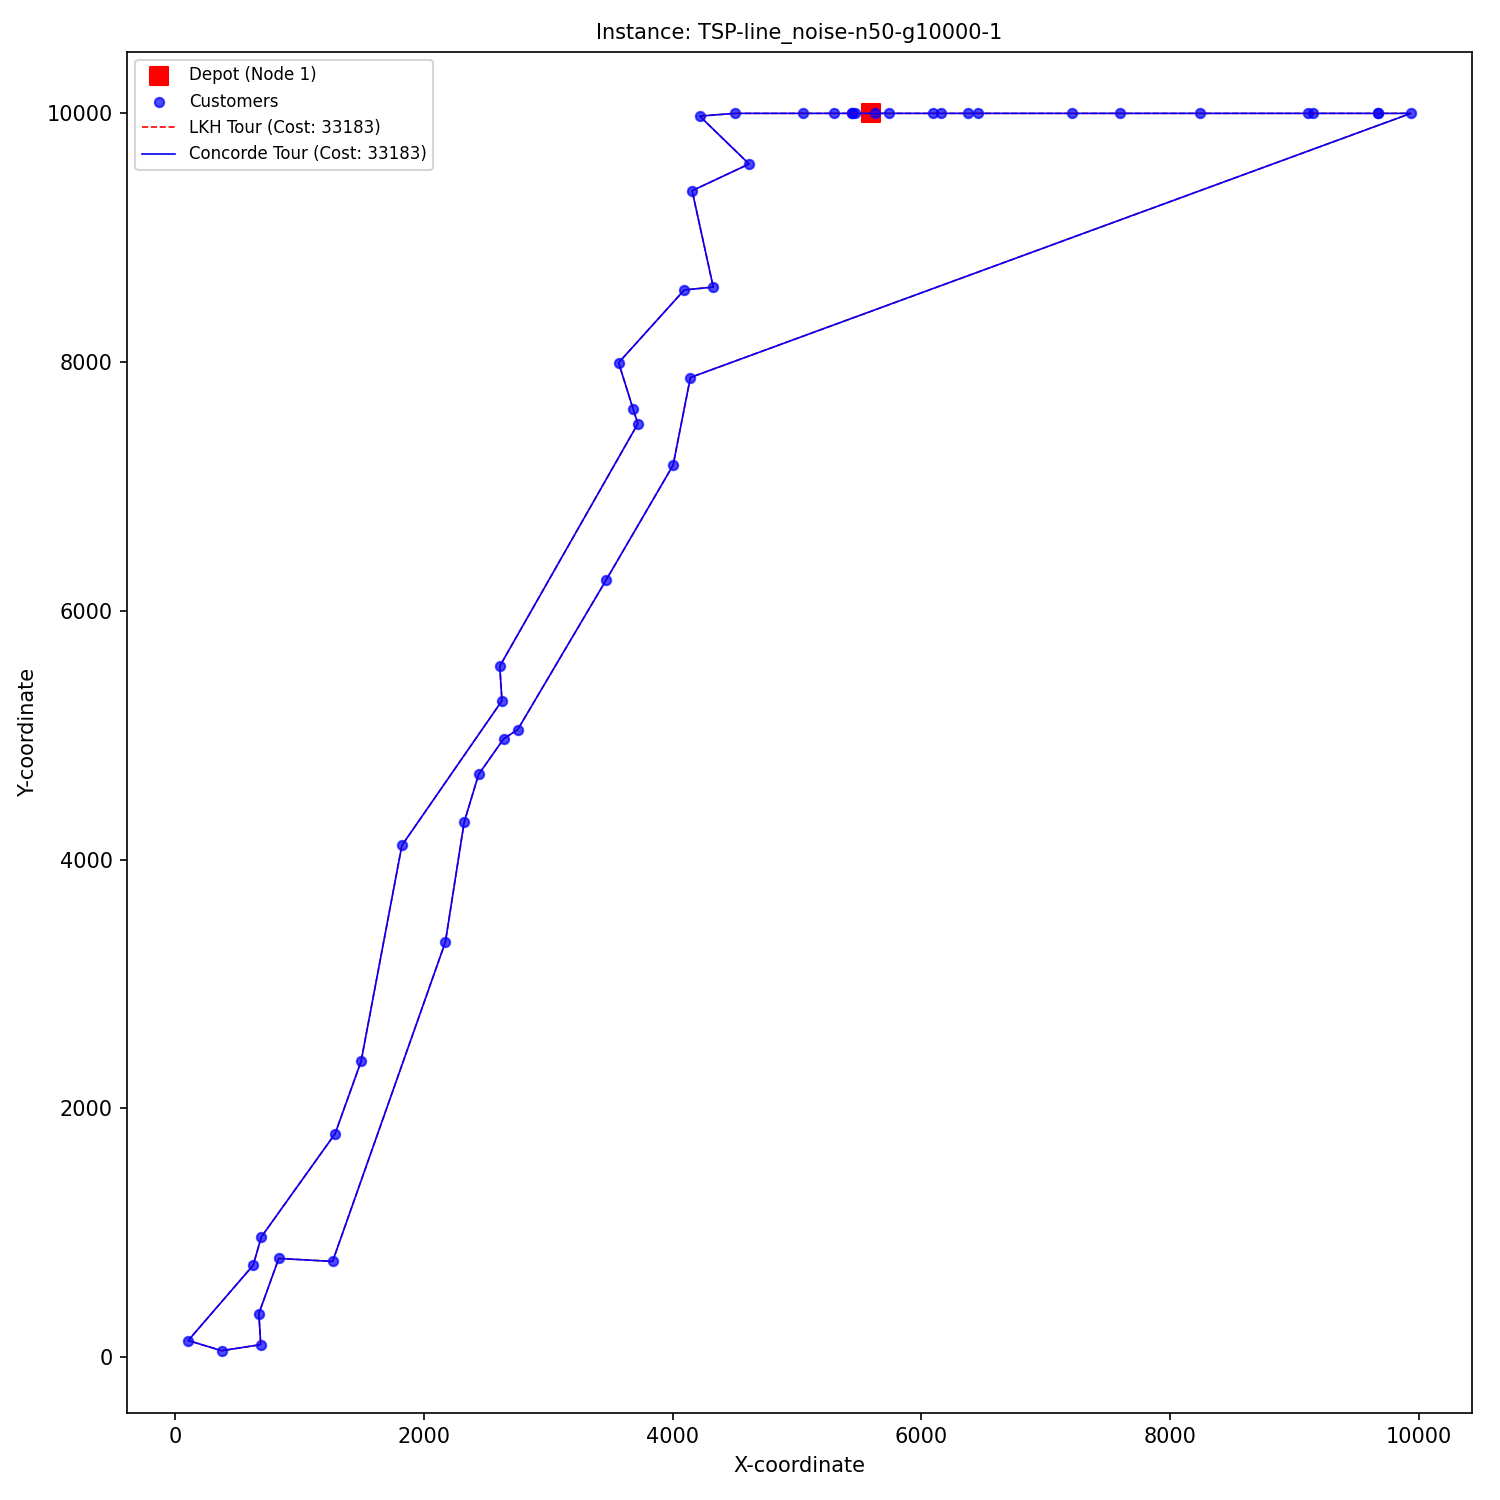
\includegraphics[width=0.6\linewidth]{TSP-line_noise-n50-g10000-1.png}
    \caption{Adversarial Line Noise Instance ($N=50$)}
    \label{fig:line_noise_example}
\end{figure}

We quantified the impact of this distributional shift using Levene's Test for Equality of Variances. The null hypothesis posits that the variance of the percentage error remains constant between the standard 2D benchmark and the Line Noise dataset. As shown in Table \ref{tab:levene_test}, every evaluated model rejected the null hypothesis with $p$-values effectively at zero ($p < 10^{-6}$). This indicates a significant decline in variance across all surveyed models.

\begin{table}[ht]
\centering
\caption{Levene's Test for Variance Stability (Standard vs. Line Noise). The extremely low p-values indicate that all models exhibit statistically significant performance degradation or alteration when exposed to linear topologies.}
\label{tab:levene_test}
\resizebox{\textwidth}{!}{%
\begin{tabular}{@{}lc|lc@{}}
\toprule
\textbf{Model} & \textbf{Levene $p$-value} & \textbf{Model} & \textbf{Levene $p$-value} \\ \midrule
Basel\_Willemain & $1.48 \times 10^{-25}$ & \textbf{GART 3.0 (V3)} & $1.23 \times 10^{-19}$ \\
Chien & $5.97 \times 10^{-23}$ & Lasso Poly V3 & $1.44 \times 10^{-17}$ \\
NN v4 (Varol) & $7.66 \times 10^{-23}$ & MST Ratio & $2.05 \times 10^{-07}$ \\
Cavdar & $3.71 \times 10^{-21}$ & \textbf{GART 1.0}& $8.28 \times 10^{-06}$ \\
BHH Asymptotic & $2.05 \times 10^{-10}$ & Linear & $2.20 \times 10^{-09}$ \\ \bottomrule
\end{tabular}%
}
\end{table}

\subsubsection{GART 1.0 vs. GART 3.0}
A critical comparison lies between GART 1.0, which utilizes the exact Convex Hull ($\phi_{Hull}$), and GART 3.0, which relies on topological proxies ($\phi_{MST}$). Theoretically, the explicit Convex Hull should provide GART 1.0 with a "ground truth" boundary, making it resilient to the emptiness of the bounding box ($A_{box}$).

However, the results in Table \ref{tab:levene_test} refute this hypothesis. GART 1.0 rejected the null hypothesis ($p \approx 10^{-6}$), confirming that it was not resilient to the adversarial topology. Despite having access to the precise volume of the point cloud, the model failed to generalize its learned relationships from the training set (Uniform/Clustered) to the linear manifold. 

This outcome demonstrates that feature engineering alone even including high quality geometric descriptors like the Convex Hull is insufficient to guarantee robustness against unseen topologies. The failure of both GART 1.0 and GART 3.0 suggests that future iterations must address this gap not merely through better features, but by actively including adversarial topologies in the training curriculum to allow the models to learn the specific failure modes of bounding-box assumptions.
\section{Conclusion}
\label{sec:conclusion}

This study set out to bridge the gap between classical 2D heuristics and the requirements of modern high-dimensional optimization. By generalizing the tour length estimation problem to $\mathbb{R}^N$, we demonstrated that the historical reliance on geometric bounding boxes, while sufficient for planar logistics, is a dead end for higher-dimensional abstract spaces.

\subsection{Summary of Findings}
Our results establish GART 3.0 as a robust, scalable estimator for the N-dimensional Traveling Salesman Problem.
\begin{itemize}
    \item Computational Scalability\textbf{:} GART 3.0 achieves a 732x average speedup over exact solvers on standard benchmarks ($N=1000, d=5$). Unlike geometric estimators which rely on the computationally expensive Convex Hull ($O(N^{\lfloor d/2 \rfloor})$), GART 3.0 utilizes a dimension-agnostic topological feature set ($\mathcal{F}_{Topo}$) that scales quadratically $O(N^2)$, ensuring viability even in hyper-dimensional feature spaces.
    \item Precision vs. Complexity: The model achieves a predictive precision of **SDPE = 1.59\%** on unseen test data, matching or exceeding the performance of deep neural networks (SDPE = 1.66\%) while requiring significantly less inference time. This confirms that Gradient Boosted Trees, when fed topologically rich features like the MST spectrum, can approximate the NP-hard TSP functional as effectively as complex differentiable manifolds.
    \item We identified a non-trivial trade-off in low dimensions. In $\mathbb{R}^2$, the explicit Convex Hull used by GART 1.0 is computationally cheaper and geometrically stricter than the MST proxies used by GART 3.0. The dataset did not include sufficiently high dimensions to find the tradeoff point where the value of using the additional features outweighed their cost.
\end{itemize}

\subsection{Limitations and Future Work}
The adversarial analysis on the "Line Noise" dataset exposed a critical limitation in the current state of the art.
\begin{enumerate}
    \item Topological Blind Spots: The universal failure of all estimators (including GART 1.0 with Convex Hull) to correctly predict linear topologies indicates that feature engineering alone is insufficient. The models "hallucinated" volume where none existed. Future work must design unique challenging topologies, explicitly including anisotropic and manifold-degenerate distributions in the training data to improve performance.
    \item Hyper-Dimensional Validation: While our theoretical derivation ensures GART 3.0 is valid for any $d$, our ground-truth validation was limited to $d \le 5$ due to computational limitations. Future research should leverage high-quality lower bounds (e.g., Held-Karp relaxations) to benchmark performance in dimensions $d=50$ to $d=100$, relevant for semantic NLP vectors.
\end{enumerate}

In conclusion, GART 3.0 provides a critical tool for "pseudo-TSP" problems in bioinformatics and data science. By decoupling estimation from Euclidean intuition, it allows researchers to treat abstract similarity metrics as geometric tours, enabling improved optimization in those spaces where human intuition.

%Bibliography
\newpage
\bibliographystyle{unsrt}  
\bibliography{references}  


\end{document}
